%!TEX root = ../thesis.tex
%Adding the above line, with the name of your base .tex file (in this case "thesis.tex") will allow you to compile the whole thesis even when working inside one of the chapter tex files

\singlespacing
\chapter{Coronal Mass Ejection Masses, Energetics, and Forces} 
\label{chap:4}
\vspace{-10mm}
\doublespacing
In the past, measurement of CME dynamics have been hindered by highly uncertain estimates of the total mass of the ejection. The primary source of uncertainty is the unknown position and geometry of the CME, leading to an erroneous treatment of the Thomson scattering equations which are used to estimate the mass. Geometrical uncertainty on the CMEs position and size has primarily been due to observations of the eruption from a single vantage point. However, with the launch of the {\it Solar Terrestrial Relations Observatory (STEREO)} mission, the two viewpoints can be exploited to derive the CMEs position and size, ultimately resulting in mass uncertainty that is both reliably quantified and much reduced. This then leads to better estimates of the energies and forces. This chapter will first outline the Thomson scattering theory used to compute CME mass, followed by a discussion of the mass uncertainties. This is followed by results showing the smallest uncertainties in the literature on CME mass, and the first estimate CME force magnitude from observations. This chapter is based on work published in Carley, McAteer, \& Gallagher, {\it The Astrophysical Journal}, 2012.

\section{Introduction}\label{sec:1}

Despite many years of study, the origin of the forces that drive coronal mass ejections (CMEs) in the solar corona and interplanetary space are not well understood. From an observational viewpoint a complete understanding of CME kinematics, dynamics and forces requires not only a study of CME speed, acceleration and expansion but also an accurate knowledge of CME mass.  The measurements of CME mass combined with acceleration measurements can be used to quantify the magnitude of the force that drives a CME. Knowledge of this force magnitude can lead to an identification of the possible origin of the CME driver. 

There are numerous theoretical models that attempt to explain the triggering of CME eruption and its consequent propagation. Each describe the destabilization and propagation of a complex magnetic structure, such as a flux rope, via mechanisms that include the catastrophe model \citep{forbes1991,forbes1995,lin2000}, magnetic breakout model \citep{antio99,lynch2008}, or a toroidal instability model \citep{chen1996,kleim2006}, as described in Chapter 2. The loss of equilibrium induced by such mechanisms results in CME propagation into interplanetary space. The predictions of these models have been investigated in observational studies whereby the CME kinematics are used to constrain what forces might be at play and hence which model best describes CME propagation. Such studies show that early phase propagation can be reasonably described by the existing models (or a combination of them) involving some form of magnetic CME driver \citep{manoh2003, chen2006, schrijver2008c, lin2010}, and that aerodynamic drag of the solar wind may have a significant role at later stages of CME propagation \citep{howard2007, malo10, byrne2010}. Comparisons between modeling and observational estimates of the forces that drive CMEs requires an accurate determination of CME kinematics properties as well as CME mass.

To date, the most prevalent method of determining CME mass has been through the use of white light coronagraph imagers, such as the Large Angle Spectroscopic Coronagraph  \citep[LASCO;][]{bru95} on board the \emph{Solar and Heliospheric Observatory} \citep[\emph{SOHO};][]{dom95}  and the twin Sun Earth Connection Coronal and Heliospheric Investigation (SECCHI) COR1 and COR2 coronagraphs \citep{how08} on board the \emph{Solar Terrestrial Relations Observatory}  \citep[\emph{STEREO};][]{kai08}. The white-light emission imaged by such coronagraphs occurs via Thomson scattering of photospheric light by coronal electrons \citep{min30, vdeh50, bil66}, the so called K-corona.  From classical Thomson scattering theory, the intensity of the light detected by an observer depends on the particle density of the scattering plasma. Hence, any density enhancement, such as a CME, over the background coronal density appears as enhanced emission in white light. The enhanced emission allows for a calculation of the total electron content and hence mass. 

Some of the first measurements of CME mass using scattering theory were carried out by \citet{munro1979} and \citet{poland1981} using space-based white light coronagraphs on board \emph{SkyLab} and U.S. military satellite\,\emph{P78-1}.  Both the early studies  and later statistical investigations determined that the majority of CMEs have masses in the range of 10$^{13}$--10$^{16}$\,g, \citep{vourlidas02, vour2010}. However, due to only a single viewpoint of observation, the longitudinal angle at which the CME propagates outwards was largely unknown in these studies 
and it is generally assumed that the CME propagates perpendicular to the observers line-of-sight (LOS). There is also the added assumption that all CME mass lies in the two-dimensional plane-of-sky (POS). Such assumptions can lead to a mass underestimation of up to 50\% or more \citep{vou00}. More recent studies have employed the two viewpoint capabilities of the \emph{STEREO} mission to determine the mass of numerous 
CMEs with much less uncertainty \citep{cola09}. 
	
This Chapter presents an analysis of mass development of the 2008 December 12 CME using the \emph{STEREO} COR1 and COR2 coronagraphs. We use a well constrained angle of propagation to determine the mass and position of the CM, and completely characterise the uncertainties on this mass. Combining the mass measurements with values for CME velocity and acceleration, the kinetic energy and the magnitude of the force influencing propagation is determined for each point in time. The first section described the observations of the event from first appearance of the front in COR1 A and B to the time when the front exits the COR2 A and B fields of view. 
The data analysis section describes the methods by which the masses are calculated with \emph{a priori} knowledge of the propagation angle, as well as a discussion of the primary sources of uncertainty. Following this are the results, including masses, energies and forces on the CME. Finally, a discussion is given of the possible forces attributable to the observed accelerations and whether they are magnetic or aerodynamic in origin. 

\section{Observations}

The COR1 images used in this analysis span from 2008 December 12 04:05\,UT to 15:45\,UT, with a cadence of 10\,minutes. The three polarization states of COR1 were combined to make total brightness images in units of mean solar brightness (MSB). Base difference images were produced using the 04:05\,UT image (in both COR1\,A\,and\,B) as a background to be subtracted from all subsequent images. A sample of such images for both COR1\,A and B can be found in Figure~\ref{fig:STEREO_COR1A&B}. The COR2 images analyzed range from from 07:22\,UT to 17:52\,UT, with a cadence of 30\,minutes. As with the COR1 images, total brightness images were created for COR2, and a set of base difference images were then produced using the 07:22\,UT image as a suitable background. A selected set of images from COR2 can be found in Figure~\ref{fig:STEREO_COR2A&B}. Note that the pixel values in Figures~\ref{fig:STEREO_COR1A&B} and~\ref{fig:STEREO_COR2A&B}  have been converted to grams; the method by which this is done is described in the next section.
	
At 04:35\,UT the leading edge of a CME appeared in COR1\,A and B coronagraphs at a height of $\sim$1.4\,$R_{\odot}$, off the east and west limb respectively. In COR1\,B the CME first appears as a set of rising loop-like structures followed by a prominence, part of which appears to fall back to the surface at 08:00\,UT while the remainder was ejected and follows the rising loop-like structures which eventually become the CME front. The rising prominence was not apparent at any stage of the propagation in COR1\,A and the advancing front remains the only distinguishable facet 
of the CME from this line-of-sight (LOS).
\begin{sidewaysfigure}
    \centering
	\includegraphics[scale=0.6]{cor1ab_color.pdf}
	\caption [2008-December-12 CME observed by COR1] {Selection of base difference images of the CME in COR1\,A  
	(top row) and COR1\,B (bottom row). The CME is quite faint in the A images and appears not to have as much structure
	as in B. As indicated by the color bar on the right, this image has units of grams. The method by which pixel units of 		grams are derived is described below.}
\label{fig:STEREO_COR1A&B}
\end{sidewaysfigure}

\begin{sidewaysfigure}
    \centering
    \includegraphics[scale=0.8, trim=0cm 3cm 0cm 1cm]{cor2ab_color_test.pdf}
	\caption [2008-December-12 CMe observed by COR2]{Selection of base difference images of the CME in COR2\,A (top 	row) and COR2\,B (bottom row). The CME is 
	clearly distinguishable in both fields of view. Only the B field view shows clearly the three part structure of core, cavity 	and front. As with the COR1 images these images also have units of grams; the method by which grams are calculated is described below.}
\label{fig:STEREO_COR2A&B}
\end{sidewaysfigure}    

A noteworthy caveat of using base difference imaging is the assumption that the background corona in the pre-event image has the same brightness in all subsequent images. This may not always be true and any excess brightness in the pre-event image will produce negative pixel values in the base difference. This is apparent in the COR1 images as the CME interacts with a streamer, displacing it as the leading CME front expands laterally as well as moves outward. The streamer is visible as a dark feature that grows with time at the southward flank of the CME in the COR1\,B images, Figure~\ref{fig:STEREO_COR1A&B}. The black areas are indicative of negative pixel values. The COR1\,A images also suffer from negative pixels, especially at later times, see Figure~\ref{fig:STEREO_COR1A&B} top row, 09:15\,UT image. 
The front of the CME starts to exit both the A and B field of view at $\sim$08:35\,UT.

The CME first appears in the COR2 field of view at $\sim$07:52\,UT with the CME apex at a height of $\sim$3\,$R_{\odot}$ in both A and B images. In the B coronagraph, by 10:52\,UT the three part structure of core, cavity, and bright front is clearly visible and the overall structure grows in size as the CME propagates to larger heights. The core becomes more tenuous and the mass distribution becomes homogenous after 15:52\,UT when the front starts to exit the field of view. The distinction between core and front is not as clear in COR2\,A and the mass distribution appears more homogenous throughout the propagation. As with the COR1 images, COR2\,A is also affected by excess brightness in the pre-event image, as is apparent by a growing dark feature in its southern half. As the pre-event image for COR2\,B is the cleanest of the pre-event images (it contains the least contamination by streamers), the COR2\,B data are considered the best candidate for accurate CME mass measurements. 



\section{Data Analysis}\label{sec:10}

As mentioned, a CME is visible through the Thomson scattering of photospheric light by all electrons in the CME.
A conversion from pixel units of mean solar brightness to grams requires a knowledge of how electrons scatter photospheric light in the corona. Before discussing how CME masses are calculated, a brief overview of Thomson scattering theory is given here, along with a discussion of the uncertainties due to some unknowns about the CME position and shape.

\subsection{Thomson Scattering in the Corona}\label{sec:10}
\doublespacing
Thomson scattering involves an incident electromagnetic wave exciting an oscillation of an electron such that the electron radiates like a small dipole. In this way some of the incident electromagnetic energy is `scattered' in a variety of directions, given by the radiation pattern of the oscillating electron. Any incident radiation falling on the area
\begin{equation}
\sigma_T = \frac{8\pi}{3}\bigg(  \frac{e^2}{4\pi\epsilon_0 m_e c^2}   \bigg)^2 = \frac{8\pi}{3}r_e^2 = 6.65\times10^{-29}\,\mathrm{m}^2
\end{equation}
will be scattered by the electron into a dipole radiation pattern. $r_e$ is the classical electron radius, $e$ is electron charge, $m_e$ is electron mass, $c$ is the speed of light, $\epsilon_0$ os the electric permittivity of free space. The area is the Thomson scattering cross-section and is independent of wavelength of the incident wave; all wavelengths are scattered equally. 

\begin{figure}[!t]
\begin{center}
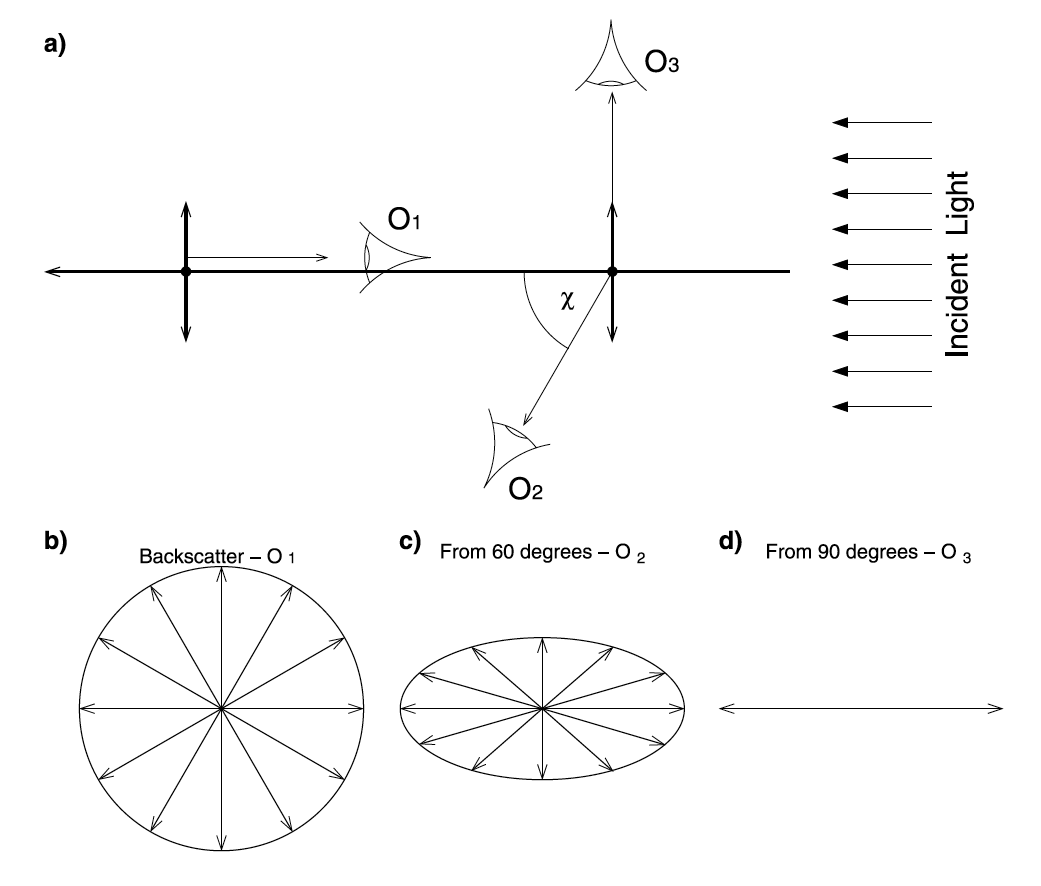
\includegraphics[scale=0.35, trim=1cm 0cm 0cm 0cm]{t_scatter}
\caption[Thomson scattering schematic.]{Thomson scattering schematic geometry in three dimensions. The incident light is unpolarised and sets the electron into oscillation in directions out of the plane of the page and parallel to it, (a) shows the viewing angles relative to incident radiation. O$_1$ shows a viewing angle at $0^{\circ}$ or $180^{\circ}$ and the directions of oscillations seen by the observer (b) -- this is completely unpolarised radiation. (c) shows a viewing angle of $\chi$, where the oscillation in the plane of the page is foreshortened, resulting in partially polarised light. (d) shows viewing angles of $\chi=90^{\circ}$, which is linearly polarised \citep{howtap2009}.}
\label{fig:tscatter}
\end{center}
\end{figure}
Solar photospheric radiation is completely unpolarized, hence the radiation incident on a coronal electron with set it into an oscillation with an amplitude that is equal in all directions. In Figure ~\ref{fig:tscatter}, their are two components to the incoming light, setting the electron into oscillation parallel to the page and perpendicular to it. No matter what the viewing angle, $\chi$, the perpendicular oscillation will always be observed to have the same amplitude. However, the parallel component will be fore-shortened, depending on $\chi$. In this way, the radiation may appear unpolarized (Figure~\ref{fig:tscatter}(b)), partially polarized (Figure~\ref{fig:tscatter}(c)), or completely linearly polarized (Figure~\ref{fig:tscatter}(d)).

\citet{schuster1879} and \citet{minnaert1930} were the first to formalise the Thomson scattering theory for an electron in the solar atmosphere. The electron is set into oscillation by an unpolarized  incident intensity $I_0$.
The two components of radiation observed are the tangential component, $I_T$ in the plane perpendicular to the page, and radial component, $I_R$ in the plane of the page Figure~\ref{fig:omega}. 
These two components are given by the expressions \citep{howtap2009}
\begin{eqnarray}
I_T &=& I_0\frac{\pi \sigma_e}{2z^2}[(1-u)C +uD] \\
I_P &=& I_0\frac{\pi \sigma_e}{2z^2}\mathrm{sin}^2\chi[(1-u)A +uB] \\
I_R &=& I_T-I_P
\end{eqnarray}
where $I_0$ is incident intensity, $\sigma_e$ is the electron scattering cross section, $z$ is the distance from scatterer to observer, $u$ is a limb darkening coefficient. $I_R$ is given via a polarization intensity $I_P$ for ease of derivation. These equations describe theoretically the concepts outlined in Figure~\ref{fig:tscatter} e.g, both $I_T$ and $I_R$ are fully observed at $\chi=0^{\circ}$ and $\chi=180^{\circ}$, while only $I_T$ is observed at $\chi=90^{\circ}$. 
\begin{figure}[!t]
\begin{center}
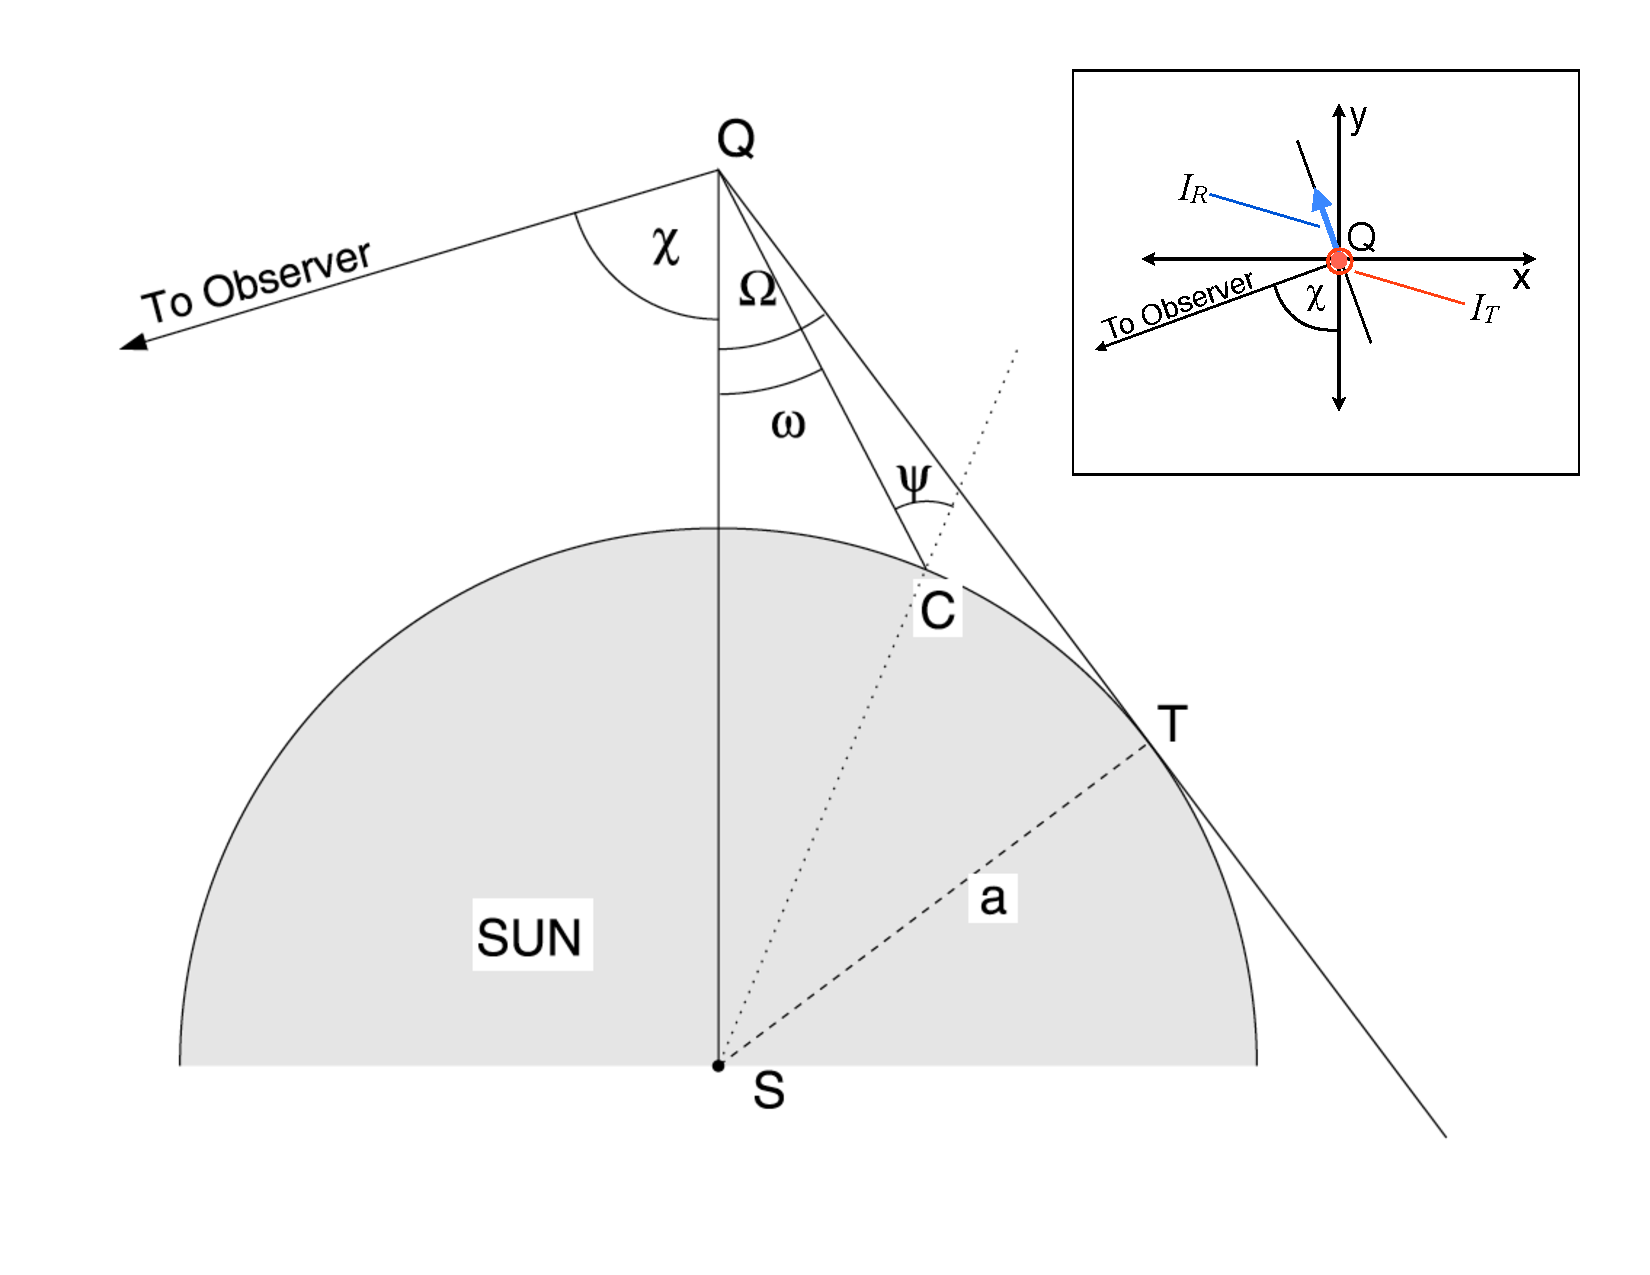
\includegraphics[scale=0.5, trim=0cm 2cm 0cm 0cm]{omega_new.pdf}
\caption[Thomson scattering geometry in the solar corona]{Thomson scattering geometry in the solar corona. The orientation of $I_R$ and $I_T$ is shown in the inset. $I_R$ is the projection of electron oscillation in the x direction onto a plane perpendicular to the line from Q to observer. $I_R$ is zero when $\chi=90$. $I_T$ is due to electron oscillation out of the plane of the page (z-direction), and is completely unaffected by viewing angle. Figure adapted from Figure 3 of \citep{howtap2009}.}
\label{fig:omega}
\end{center}
\end{figure}
The main complication for Thomson scattering by a coronal electron is that the Sun is not a point source. The effects of the finite size of the Sun are incorporated into $A$, $B$, $C$, and $D$ in equations (4.2)--(4.4). These are trigonometric expressions known as the van de Hulst coefficients \citep{vdeh50}, and completely characterise the reception of light by the electron from across the entire solar disk, using only the angle $\Omega$, the angle subtended by the solar disk from point Q shown in Figure~\ref{fig:omega} \citep{minnaert1930, billings1966, billings1966} 
\begin{eqnarray}
A &=& \cos \Omega \sin^2 \Omega \\
%
B &=& -\frac{1}{8}\bigg[1 - 3\sin^2\Omega -\frac{\cos^2\Omega}{\sin\Omega}(1+3\sin^2\Omega)\textrm{ln}\bigg(\frac{1+\sin\Omega}{\cos\Omega}\bigg)\bigg] \\
%
C &=& \frac{4}{3} - \cos\Omega - \frac{\cos^3\Omega}{3} \\
%
D &=& \frac{1}{8}\bigg[5 + \sin^2\Omega -\frac{\cos^2\Omega}{\sin\Omega}(5-\sin^2\Omega)\textrm{ln}\bigg(\frac{1+\sin\Omega}{\cos\Omega}\bigg)\bigg] 
\end{eqnarray}
Each electron in a CME will scatter light according to equations (4.2)--(4.8). They described light scattered by an electron at any position in the solar atmosphere (any $\Omega$), with the observer at viewing angle $\chi$. The intensities given by these equations are for a single electron. If there is a number of electrons $N_e$ at point Q in Figure~\ref{fig:omega}, then the intensity would simply be $IN_e$; the intensity of scattered light from a point Q depends linearly on the total number of scattering electrons at that point. Hence if we know the intensity of scattered light we may directly infer the total number electrons contributing to this intensity. This allows a calculation of the total electron content of a CME, resulting in a mass calculation. However, the intensity calculation is very sensitive to $\chi$, the viewing angle, and some important aspects of CME observation arise from this.

%As mentioned the above equations have a sensitive dependence of intensity and polarization on scattering angle $\chi$. The total intensity of scattered light is
%\begin{equation}
%I_{tot} =  2I_T - I_p \propto I_0\frac{\pi \sigma_e}{z^2}\bigg(1 - \frac{\mathrm{sin}^2\chi}{2}\bigg)
%\end{equation}
%So at $\chi=90$, $I_p$ is maximum, $I_R$ is minimum, $I_{tot}$ is minimum, and scattering efficiency is minimum. The dependency of each intensity component is shown in Figure~\ref{fig:Ivchi}. The tangential component $I_T$ remains constant at all viewing angles, whereas $I_R$ is maximum at $0^{\circ}$ or $180^{\circ}$ and minimum at $90^{\circ}$. Polarization is maximum at $90^{\circ}$. 
%\begin{figure}[!t]
%\begin{center}
%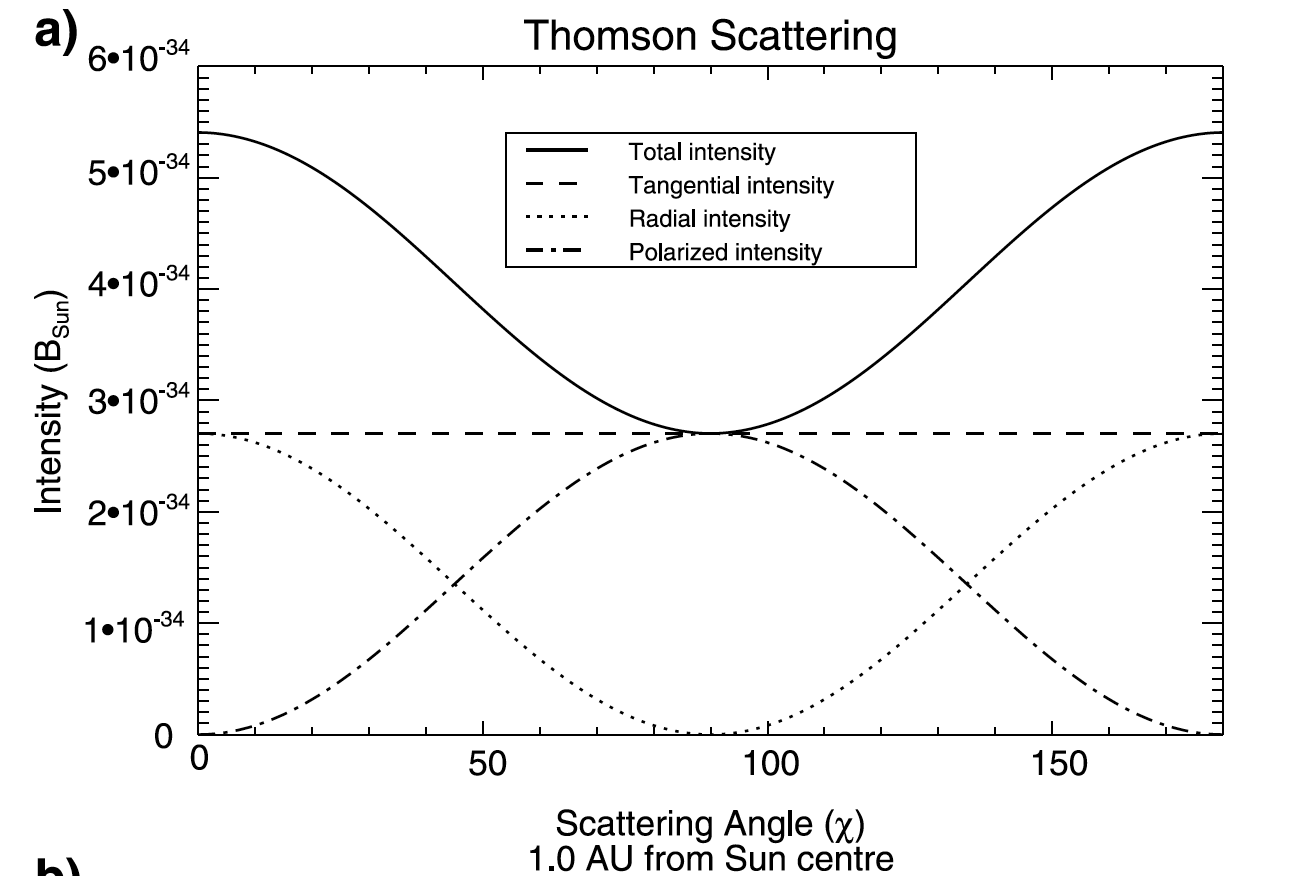
\includegraphics[scale=0.3]{IT_IR}
%\caption[Thomson scattered intensity as a function of viewing angle]{Thomson scattered intensity as a function of viewing angle.}
%\label{fig:Ivchi}
%\end{center}
%\end{figure}

Along any LOS through the corona, the point at which $\chi = 90^{\circ}$ will be the point of minimum distance from the Sun Figure~\ref{fig:LOS_POS_2}. Three effects must be considered at this point; (i) scattering efficiency is a minimum, (ii) the incident intensity ($I_0$) received from the Sun is a maximum, and (iii) the electron density is a maximum. The latter two effects, (ii)--(iii), are a bigger contributor to the scattered light than the former, (i). As a result, scattered light is maximized at the point of $\chi = 90^{\circ}$ along the line of sight, despite the efficiency of scattering being a minimum at this point. Close to the Sun, the plane making an angle of $\chi = 90^{\circ}$ with the line of sight is known as the plane-of-sky (POS) (Figure~\ref{fig:LOS_POS_2}), and is the plane of maximum scattered intensity. Any CME erupting close to the POS will be well observed. However, eruption of a CME at a large angle away from the POS will result in less scattered light from the CME electrons, making the CME appear quite faint. If the angle from the POS is unknown, there is no way of telling the amount by which the intensity is reduced. 
%Observing a smaller intensity will result in the observer calculating a smaller number of electrons contributing to the scattered light. If no correction is made for the diminished intensity, the number of electrons and hence the total CME mass will be underestimated. The correction can only be made when the angle from the POS is known. As if often the case, the angle is unknown and we must assume the CME lies on the plane of sky. If this assumption is false, there will a proportion of the CME that we will go unaccounted for, 
This can lead to an underestimation of its mass content by up to a factor of 2 \citep{vou00}. As described in the next section, unknown viewing angles, $\theta$ or $\chi$, are the largest contributor to CME mass uncertainty.


\subsection{Mass Measurement and Geometrical Uncertainties}
\begin{figure}[t!]
\begin{center}
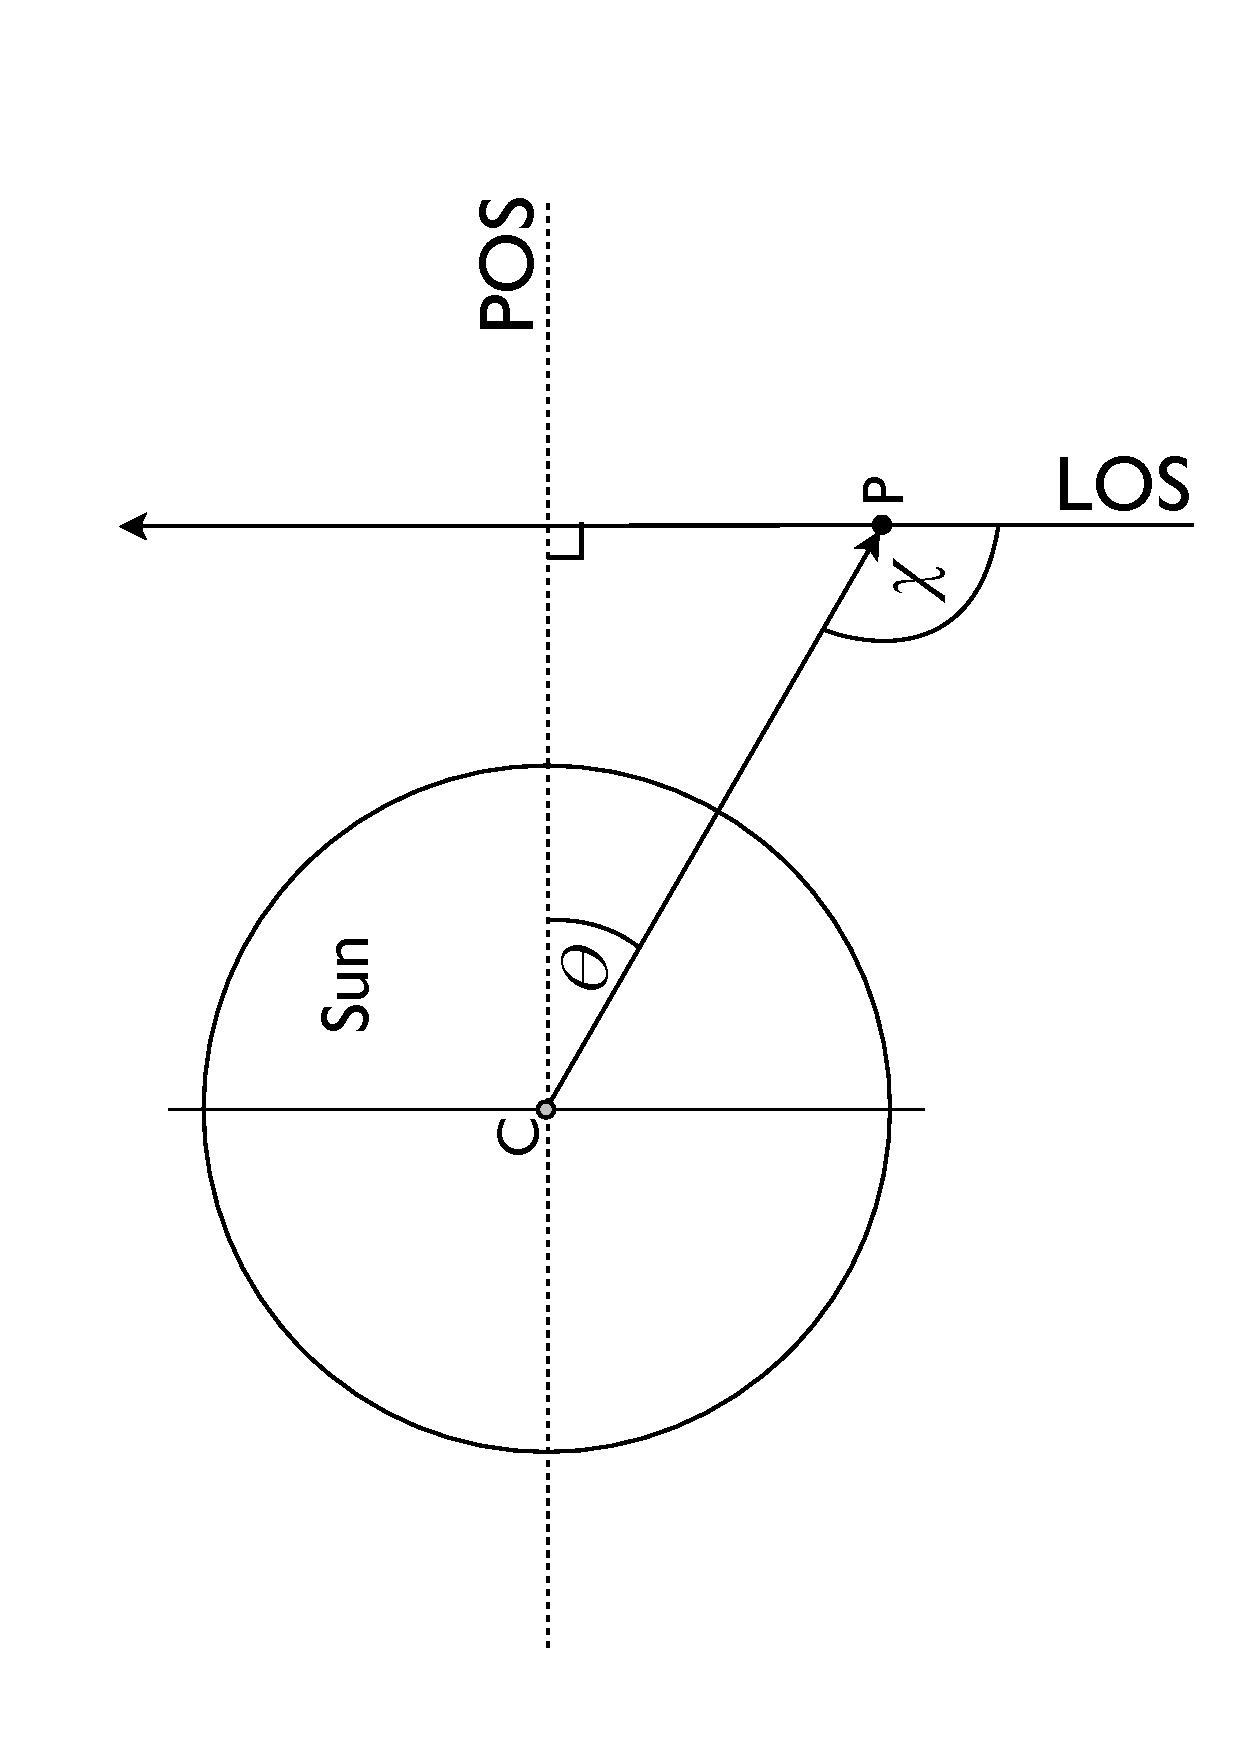
\includegraphics[trim = 0cm 0cm 0cm 0cm, scale=0.4, angle=270]{images/LOS_POS_2.pdf}
\caption[Line-of-sight and plane-of-sky orientations]{Schematic showing the relative orientation of the line-of-sight (LOS), and the plane-of-sky (POS). Electron position is at point P and C is 
Sun center. The vector CP may also represent CME propagation direction. Scattering efficiency is heavily dependent on the angle $\theta$ 
(or $\chi$) and is least efficient 
when $\theta = 0^{\circ}$ ($\chi=90^{\circ})$.}
\label{fig:LOS_POS_2}
\end{center}
\end{figure}
%
%
%
Calculating the total mass of a CME requires an estimate of the total amount of electrons contributing to the light scattered by the CME. Then assuming that the corona is 90\% hydrogen and 10\% helium, each electron will be associated with a mass of $1.97\times10^{-24}$\,g. The mass in each pixel of an image of a CME is then
\begin{equation}
m_{pixel}=\frac{I_{obs}}{I_e(\theta)} \times1.97\times10^{-24}\,\mathrm{g}
\label{eqn:mass_pix}
\end{equation}
where $I_{obs}$ is the observed pixel brightness and $I_e$ is a single electron brightness at the position that the pixel images.
The brightness $I_e(\theta)$ may be derived from the Thomson scattering equations (4.2)--(4.8), provided the angle $\theta$ from the POS is known. If not, a number of assumptions must be made about the position of the electrons along the line of sight. The primary assumptions in all CME mass measurements from white-light observations are
%------------------------------------------------------------%
%
%				   POS assumption 				  %
%
%------------------------------------------------------------%
\begin{itemize}
\item The CME propagates at right angles to the line-of-sight, along the plane-of-sky at $\theta=0$.
\item All CME electrons are confined to the plane $\theta$; the CME is a flat 2D object.
\end{itemize}
These assumption arrises because no information is available on the propagation angle of the CME with respect to the POS. 
%The assumption also implies the CME is a 2D object located on the POS, propagating at right angle to the observer's line of sight ($\theta=0$ or $\chi=90$). 
To investigate the effects of the first assumption we need only consider the CME to be a group of electrons located at some P located at angle $\theta >0^{\circ}$ from the POS (Figure~\ref{fig:LOS_POS_2}). Since for single viewpoint observations no information on $\theta$ is available, we must assume $\theta=0^{\circ}$ i.e., the electrons are located on the POS. We are assuming that each electron scatters a intensity $I_e(\theta=0^{\circ})$, when in fact it is scattering a smaller intensity of $I_e(\theta>0^{\circ})$. This means we are overestimating the contribution from each electron $I_e$, leading to an underestimate of the number of scattering electrons $n_e = I_{obs}/I_e$ in equation~\ref{eqn:mass_pix}. This will give an underestimate of the mass located at point P. 

To quantify this underestimation, we plot a single electron brightness at $\theta>0^{\circ}$ divided by the POS electron brightness, $I(\theta=0^{\circ})$, as a function of $\theta$ (Figure~\ref{fig:pos_angle}). For example, an electron located at $\theta=40^{\circ}$ will be $\sim$0.8 times as bright as an electron on the POS. Although this is for a single electron, it describes the effects of first assumption above. The CME is simply a collection of electrons at $\theta=40^{\circ}$, but we assume that the CME is at $\theta=0^{\circ}$. In such a case we only observe 80\% of the CMEs maximum brightness, but assume we are observing 100\%. In this way, we underestimate the total mass content of the CME by 20\%. This is the primary source of CME mass underestimation and it is expected that on average we underestimate total CME mass by up to a factor of 2 \citep{vou00}. For single vantage point observations there is no information about $\theta$, and, realistically, the amount by which the mass is underestimated is completely unknown.
\begin{figure}[!t]
\begin{center}
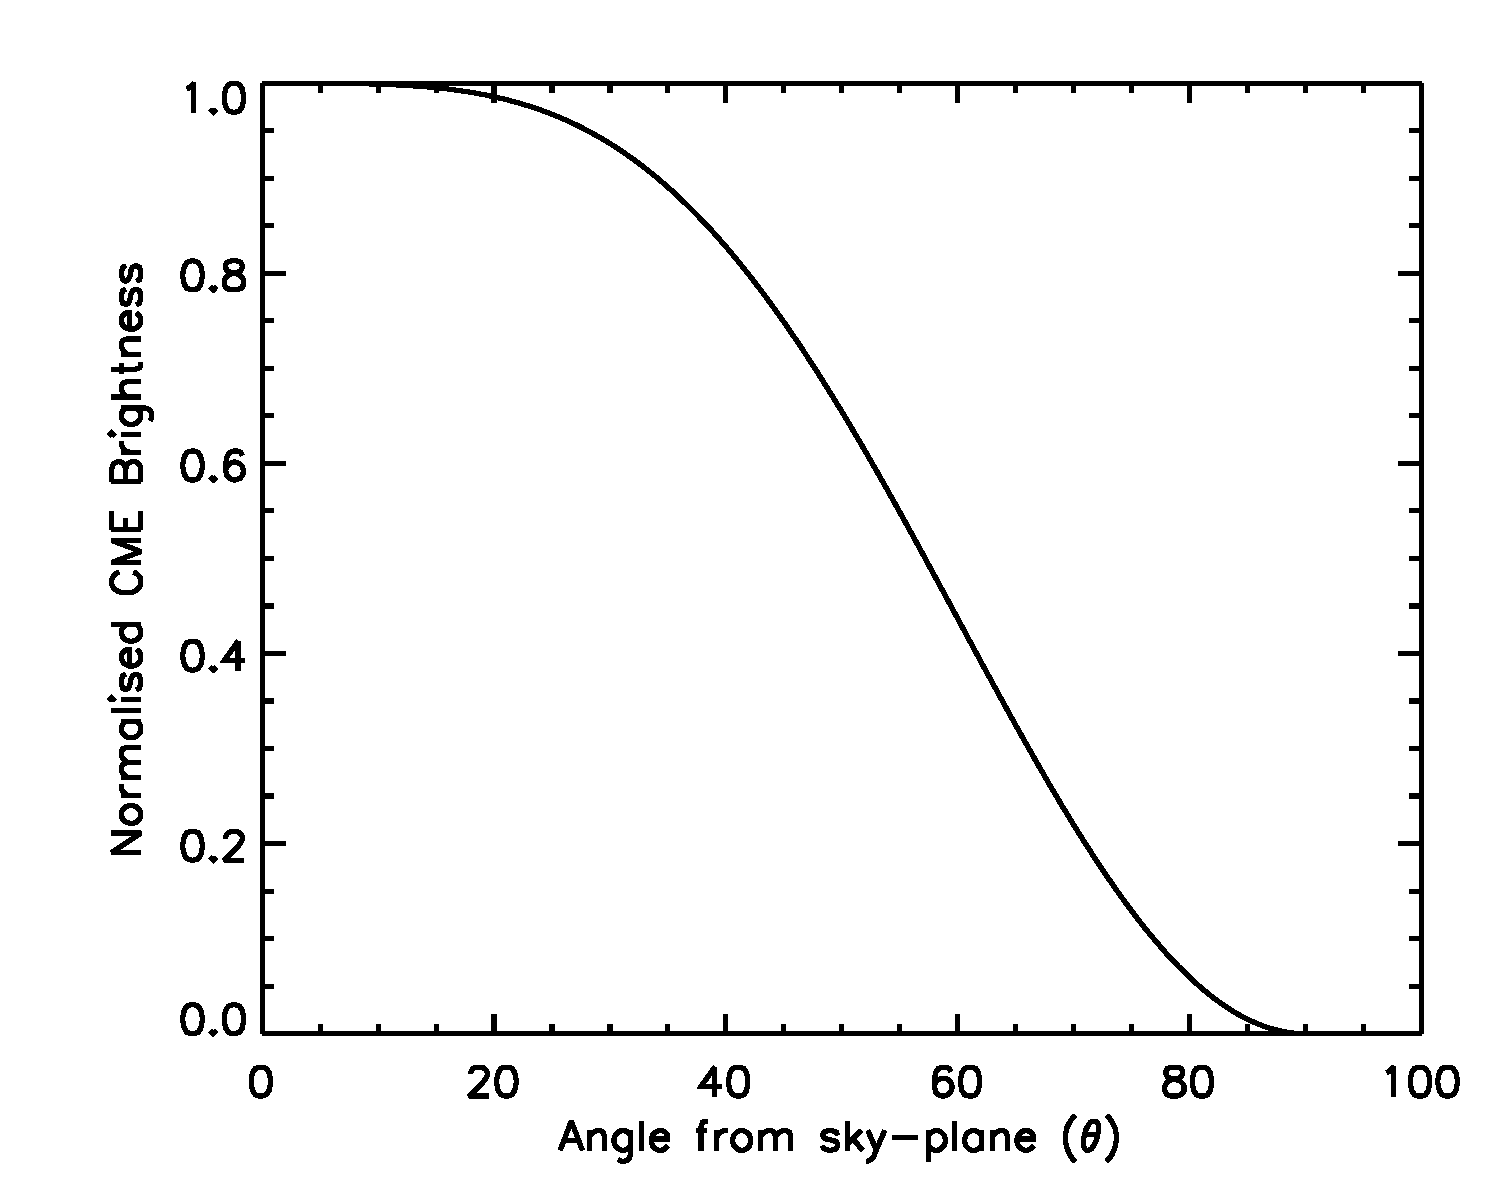
\includegraphics[scale=0.4, trim=2cm 0cm 0cm 2cm]{pos_angle.pdf}
\caption[Electron brightness as function of angle]{Normalized electron brightness ($I_e(\theta>0)/I_e(\theta=0)$) as a function of angle from POS $\theta$.}
\label{fig:pos_angle}
\end{center}
\end{figure}
%------------------------------------------------------------%
%
%				     Finite Width	 				  %
%
%------------------------------------------------------------%

The second above assumption is that all CME material lies on a 2D plane. This arrises from the fact that we do not know the distribution of CME material along the line of sight. Since the 3D extent of the CME is unknown it is also assumed that the CME is confined to the 2D sky plane. In order to quantify this, we follow the method of \citep{vou00}. This simulates the brightness of a CME with homogeneous density distribution and finite angular width $\phi$ along the LOS. We use equations the Thomson scattering equations (4.2)--(4.8) to simulated brightness of the CME and calculate a simulated observed mass by assuming that all the brightness is from electrons on the sky plane. This simulated observed mass is then compared to the actual mass as a function of CME height and width (Figure~\ref{fig:ang_width_error}).
\begin{figure}[!t]
\begin{center}
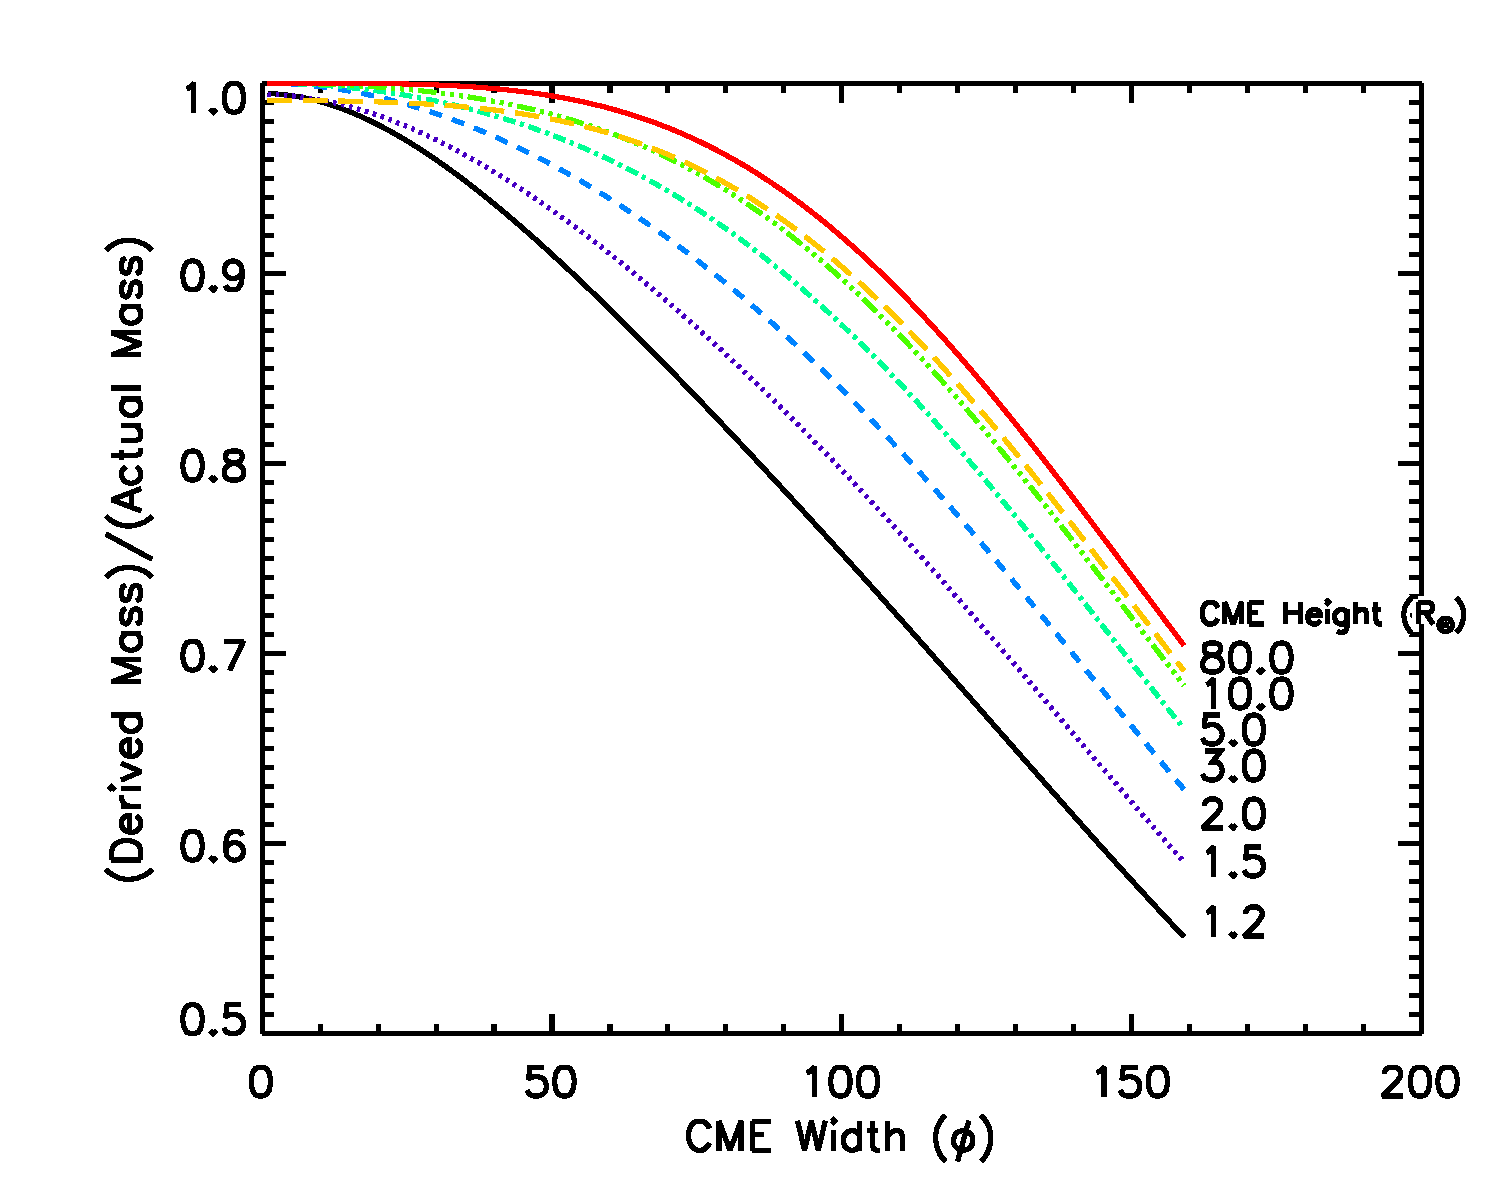
\includegraphics[scale=0.4, trim=1cm 1cm 0cm 2cm]{angular_width.pdf}
\caption[Uncertainty due to CME angular width]{CME mass underestimation as function of angular width and height. These results are from a simulated CME with height $r$, and angular width $\phi$. The simulated observed mass (derived mass) is calculated assuming that all electrons lie on the 2D POS, leading to a mass underestimation. This underestimate is quantified by comparing the derived mass with the actual mass.}
\label{fig:ang_width_error}
\end{center}
\end{figure}
For example, our assumption is that all CME material lies on the POS. However, the CME is centered on the sky-plane with angular width of $100^{\circ}$ and a height of $10\,R_{\odot}$. We will derive a mass of $\sim$0.9 of the actual mass. The underestimation arrises because all electrons are emitting their maximum brightness, when in fact some electrons are away from the sky plane and; this over-estimates the brightness contribution from those electrons, leading to an underestimate in the mass. The mass underestimation from unknown angular width is smaller than the unknown POS angle. However it can be significant for large angular widths at small heights.

Finally, we need to take into account that the CME will be propagating at some angle with respect to the POS \emph{and} have a finite angular width. To estimate the effects of this, we use the Thomson scattering theory to simulate a CME at central position angle from POS $\theta$ and width $\phi$. We derive the simulated observed mass, given the assumption that the CME is on the sky-plane, and also the assumption that the CME material is in a 2D plane at $\theta$. This simulated observed mass is compared to actual mass to derive mass underestimation in both cases.
This simulation is shown in Figure~\ref{fig:deprojection}. The dashed lines are the derived mass assuming that the CME has no angular width ($\pi=0^{\circ}$) and is on the sky-plane ($\theta=0^{\circ}$), when in fact it has finite width $\phi$ and is located at some $\theta >0$ (x-axis). The solid lines are derived mass assuming the CME lies on a 2D plane at the plane of sky angle $\theta$, this is called a 'de-projection' of the CME from the POS to its propagation plane at $\theta$. For example in Figure~\ref{fig:deprojection}(b), if the CME is at a height of $5\,R_{\odot}$, has a position angle of $40^{\circ}$, and an angular width of $120^{\circ}$, but we assume it has no width (2D) and is located on the sky-plane ($\theta=0^{\circ}$), then its derived mass will be $\sim$0.6 times the actual mass (underestimate of $\sim$40\%). If the CME is de-projected (we account for its sky-plane angle), then the derived mass is improved to a factor of 0.8 of the actual mass. Note that de-projection still assumes the CME has no width ($\phi=0$), hence there is still a mass underestimation after de-projection.
\begin{figure}[!ht]
\begin{center}
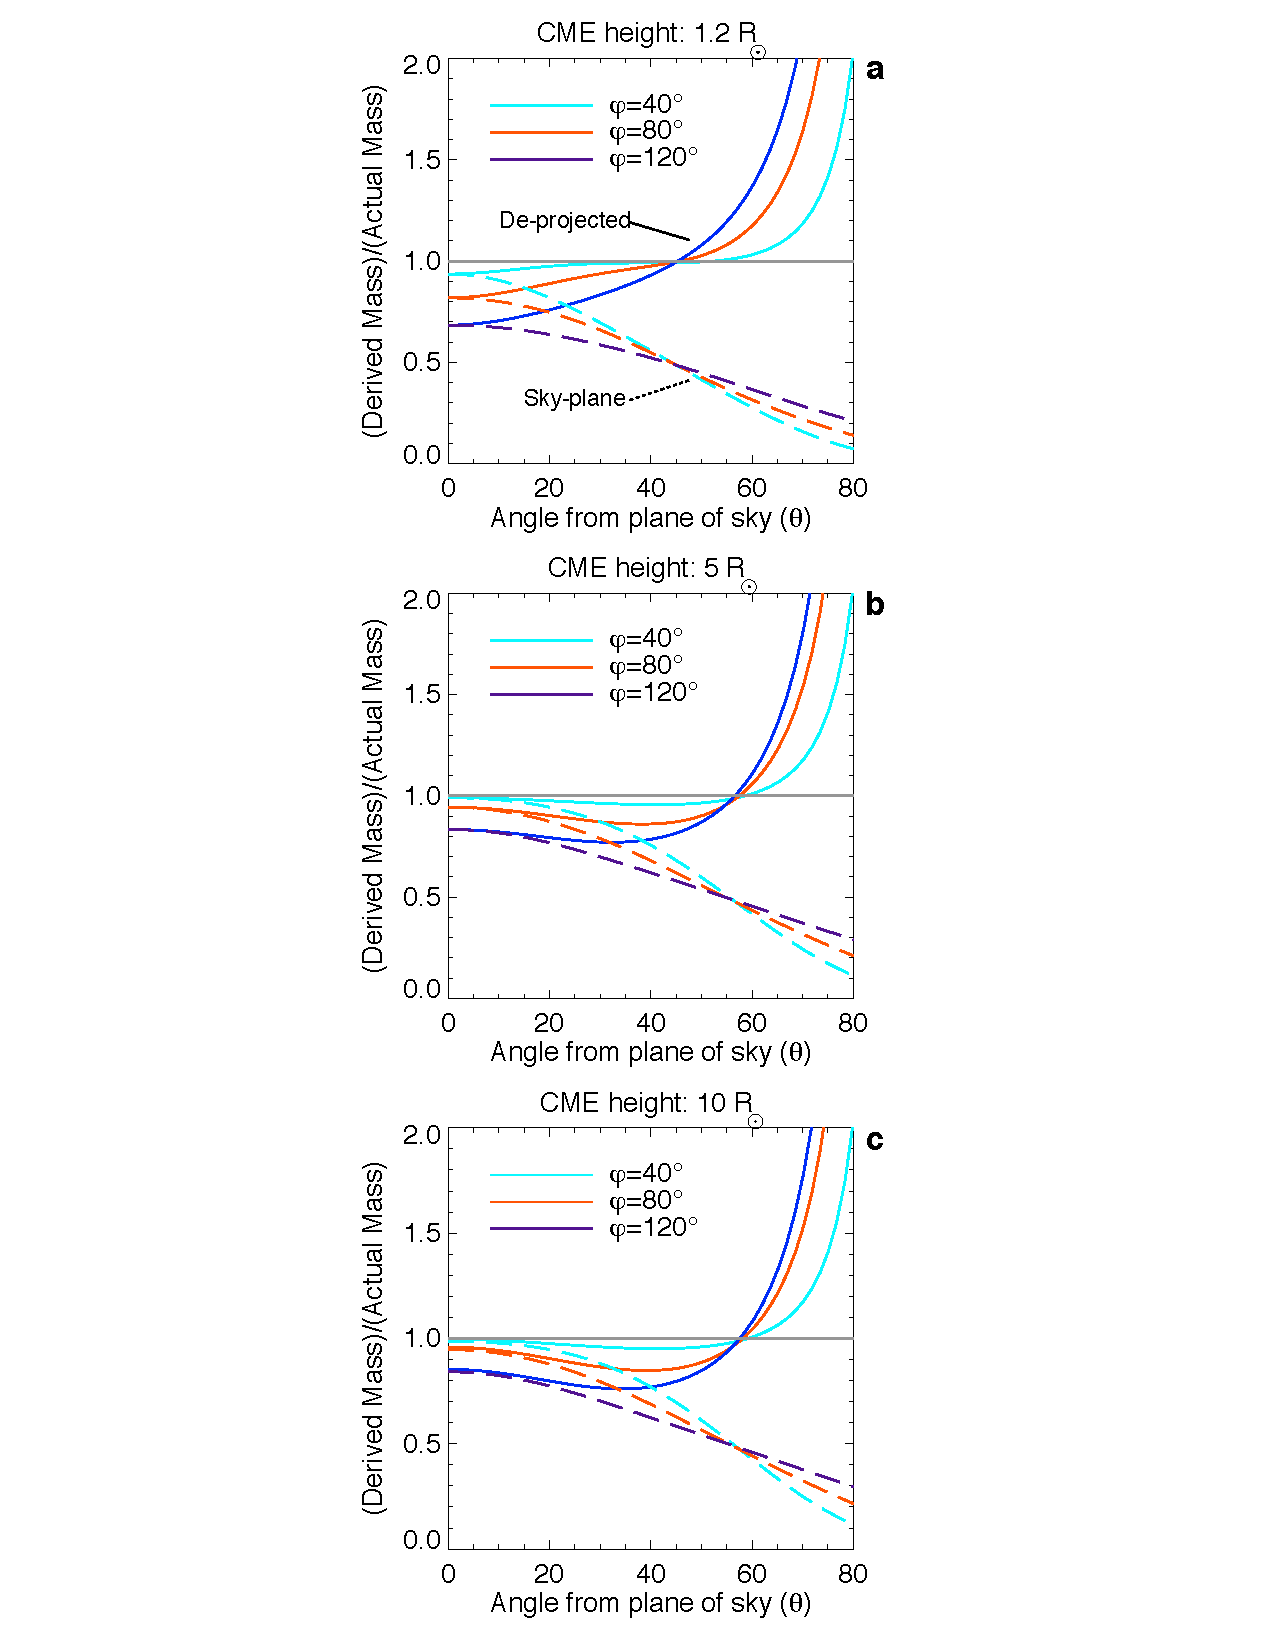
\includegraphics[scale=0.7, trim=0.5cm 0.5cm 0cm 1cm]{deprojected_pos.pdf}
\caption{Underestimation of CME mass as a function of angle from the plane of sky. The colors correspond to a CME of angular width $\phi$. Three different heights are shown. The dashed lines are mass underestimation assuming the CME has zero width ($\phi=0$) on the POS ($\theta=0$), when in fact it is has finite width of $\phi$ and is located at $\theta$ from POS. The solid lines account for the plane of sky angle $\theta$ (they are deprojected). De-projection improves the mass underestimation up to $\theta=60^{\circ}$, after which it severely overestimates the CME mass.}
\label{fig:deprojection}
\end{center}
\end{figure}
\clearpage

There is an interesting point at $\theta=~55^{\circ}$ for the $5\,R_{\odot}$ and $10\,R_{\odot}$ plots (and all larger heights). For all angular widths $\phi$, a de-projection will derive exactly the actual CME mass. Beyond this point, de-projection starts to over-estimate the CME mass and eventually overestimates it by a severe estimate at sky-plane angle greater than $70^{\circ}$. As we will see, the CME in this study had a POS angle of $45^{\circ}$ and an angular width no greater than $90^{\circ}$ for the height range of 1.4--12$R_{\odot}$. Therefore, as shown in Figure ~\ref{fig:deprojection}, a de-projection of the CME brightness to its propagation plane underestimates the mass by a smaller factor than assuming the CME is on the POS.


%---------------FROM HERE---------------------------%
\subsection{Evaluation of uncertainties}
The CME of 2008 December 12 was Earth-directed \citep{byrne2010}, making it roughly the same angular distance from both the \emph{STEREO}\,A\,and\,B spacecraft, then located $\pm$45 degrees from Earth. This known angle of propagation was used to convert from pixel values of MSB to grams via the equation~\ref{eqn:mass_pix}.
The known angle of propagation allowed the correct value of $I_{e}$ to be computed resulting in a significant reduction in the uncertainties associated with the propagation angle e.g., mass uncertainty due to the first assumption above was eradicated and the only remaining uncertainty was from the unknown finite angular width. Given that we know the de-projection angle, a measure of the angular width along the line of sight $\phi$ is needed to quantify the finite angular width uncertainty. It is possible derive the angular width along the line of sight, $\phi$, in terms of the CME latitudinal width $\psi$. We assume that $\phi \leqslant 2\psi$.  Such an upper limit is in agreement with simulations of flux-rope CMEs which give a typical aspect ratio of broadside to axial angular extents of 1.6\,--\,1.9 \citep{krall2006}. \citet{byrne2010} provided a measure of latitudinal width as a function heliocentric distance of the CME, $\psi(r)=25r^{0.22}$, giving $\phi \leqslant 50r^{0.22}$. Given that the position from the sky-plane of each spacecraft was $45^{\circ}$, and the angular widths of the CME were $<90^{\circ}$, there was a CME mass underestimation estimates of between 5--10\% for de-projected finite angular width uncertainty. Since the angular width along the line of sight is likely to be much less than $2\psi$, the 10\% uncertainty is an upper limit.


%Since the values for $\Delta$$\theta_{long}$ are unknown, the expression derived in \citet{byrne2010} for the \emph{latitudinal} angular width of this CME as a function of height, $\Delta$$\theta_{lat}$$(r)=25r^{0.22}$, was used to define an upper limit to $\Delta$$\theta_{long}$. It was assumed the CME longitudinal angular width is no more than twice the latitudinal angular width, or $\Delta$$\theta_{long}$$\leqslant$\,2$\times$$\Delta$$\theta_{lat}$. Such an upper limit is in agreement with simulations of flux-rope CMEs which give a typical aspect ratio of broadside to axial angular extents of 1.6\,--\,1.9 \citep{krall2006}. Hence the value for $\Delta$$\theta_{long}$ at each height was used to obtain the simulated mass underestimation estimates described above. The position from the sky-plane of each spacecraft was $45^{\circ}$, and given that angular widths of the CME were $<90^{\circ}$, there was a CME mass underestimation estimates of between 5--10\% for de-projected finite angular width uncertainty. An extra mass uncertainty of 6\% was added to account for the assumption of coronal abundance of 90\% hydrogen and 10\% helium which can lead to slight errors while converting from pixel values of MSB to grams \citep{vour2010}. 

Apart from the geometrical uncertainties quoted above there were a number of other minor uncertainties. The deflection of a small streamer during CME propagation produces negative pixels in the base difference images. The effect is particularly apparent in the COR1 images, Figure~\ref{fig:STEREO_COR1A&B}. It is difficult to unambiguously distinguish between streamer and CME, making it difficult to quantify the uncertainty introduced due to streamer interaction. To make an estimate of the streamer's effects, a calculation of its mass in the pre-event image was made. A number of different samples of the area of the streamer in the COR1\,B pre-event image that effects all subsequent images produced a mass estimate of $\sim$5$\times$10$^{14}$\,g. This mass was used as a measure of the uncertainty introduced due to streamer interaction in the COR1\,B images. A similar analysis of the COR1\,A pre-event images gave a streamer mass estimate of $\sim$7$\times$10$^{14}$\,g. COR2 images are relatively unaffected by significant changes in background coronal brightness and do not suffer from negative pixel values to as large an extent as COR1. The pre-event image of COR2\,B is particularly clean and free of background streamers, hence COR2\,B images are considered to provide most accurate CME mass estimation. Finally, An extra mass uncertainty of 6\% was added to account for the assumption of coronal abundance of 90\% hydrogen and 10\% helium which can lead to slight errors while converting from pixel values of MSB to grams \citep{vour2010}. 

%-----------------------------%

%-------------------PUT THIS IN KINS SECTION---------------------%
%A concise measurement of the CME kinematics, such as velocity and acceleration, were taken from the results of the study of \citet{byr10}. Since these kinematics take into account the true three dimensional surface of the front they provide reliable estimates of CME velocity and acceleration in 3-D space. These velocity and acceleration measurements were used in the calculation of kinetic energy and total force on the CME for each point in time. The CME mass used in all energy and force calculations was the asymptotic mass it approaches at later stages of its evolution beyond 10\,$R_{\odot}$ as observed from the \emph{STEREO B} spacecraft i.e.,\,3.4\,$\pm$\,1.0$\times$10$^{15}$\,g. As will be shown, there is good motivation for the use of constant mass in the magnitude of kinetic energy and force estimates. 

\section{Results}\label{sec:11}
\subsection{Masses}

To calculate the total CME mass a user-selected area (the extent of the CME, for example) of the base difference image was chosen and the pixel values within this area were summed to obtain total mass. Figure~\ref{fig:STEREO_COR2A&B} COR2 B images show an example of the sector over which pixels were summed (the smaller sectors indicate a different summing region used at a later stage). In order to obtain a more complete and continuous estimate of CME mass growth, the masses determined from both COR1 and COR2 coronagraphs were summed in those cases where image times of the inner and outer coronagraphs overlapped. This was done for each point and time to produce CME mass development with height and time

The results of the calculation for CME mass development with time and height for both \emph{STEREO} A and B coronagraphs are shown in Figure~\ref{fig:20081212_mass_ht}. In panel (a), the height values are those taken from a point-and-click method of tracking the CME apex; these heights are corrected for CME propagation angle of $\sim$$45^{\circ}$.  In both panels (a) and (b), the mass estimates of \emph{STEREO} A and B follow a similar trend and have similar values at each stage in the propagation. Such good agreement between mass values is a good indicator that $\sim$$45^{\circ}$ is the correct angle of propagation from the sky-plane. A change in the cadence of mass measurements is noticeable at $\sim$08:00 UT (or $\gtrsim$5\,$R_{\odot}$). This is due to the use of only COR1 images (with a cadence of 10\,minutes) prior to this time, and the use of the COR2 plus COR1 images after this time (the cadence of these measurements follows that of COR2\,--\,30\,minutes). Comparing A and B below 4.5\,$R_{\odot}$, mass values show a similar trend and increase at the same rate, but at approximately 3\,$R_{\odot}$ the mass measurements in COR1\,B appear to increase to a much larger value then fall again. This effect is visible in the COR1\,A measurements, albeit 
diminished. It is probably due to the presence of a prominence which contains a significant mass content and therefore contributes a large amount to total measured CME mass. Also, early on in its propagation, the prominence may still be emitting H-$\alpha$ line radiation (656.28 nm) due to the larger fraction of neutral hydrogen at its cooler temperatures.
%%%%
\begin{figure}[!t]
\begin{center}
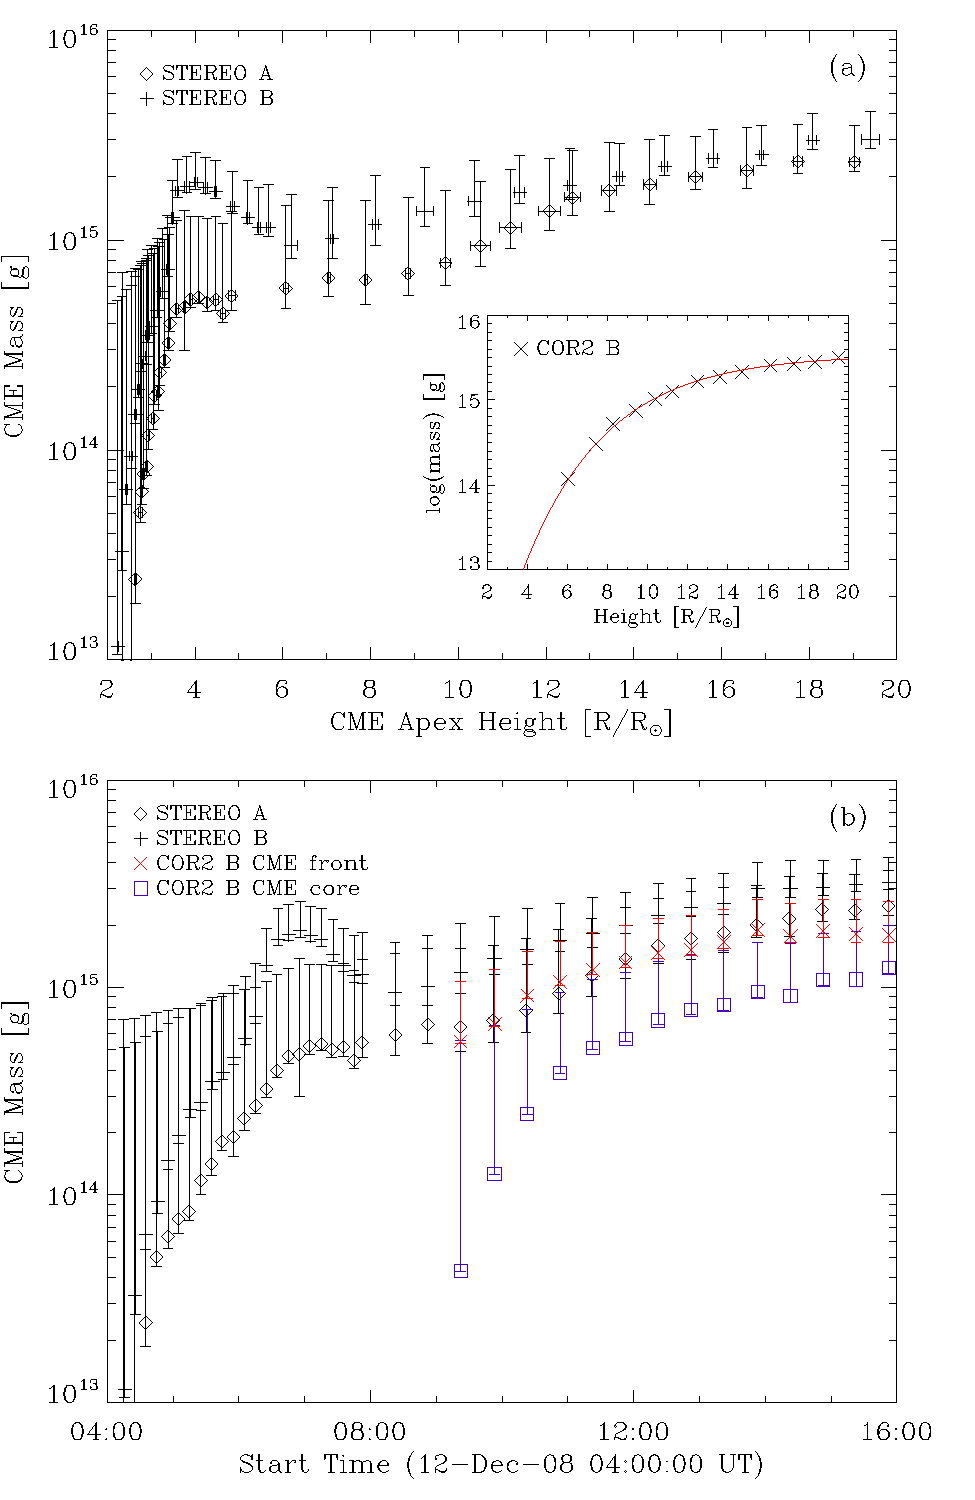
\includegraphics[scale=0.6, angle=0]{20081212_mass_ht.pdf}
\caption[CME mass as a function of height and time]{CME mass development with height (a) and time (b), for the 2008 December 12 CME. After $\sim$08:00 UT ($\gtrsim$5\,$R_{\odot}$) the masses from the inner and outer coronagraphs are summed to show uninterrupted mass development from $\sim$2--20\,$R_{\odot}$ over a period of 12 hours. The small bump in the CME mass at $\sim$07:00\,UT ($\sim$4\,$R_{\odot}$) is probably due to an unknown amount of H-$\alpha$ emission from the prominence. Mass of CME front and core are also shown, red $\textquoteleft$$\times$' and blue square, for COR2\,B, panel (b). After 14:52\,UT they share approximately equal mass. The inset of (a) shows mass development with height for COR2\,B only; the red curve represents a fit to the data whereby the mass asymptotically approaches $3.4\,\pm\,1.0\times10^{15}$\,g. }
\label{fig:20081212_mass_ht}
\end{center}
\end{figure}
%%
The COR1 imaging passband is centered on H-$\alpha$ so any emission in the prominence from neutral hydrogen could be contributing to light received by the COR1 coronagraphs, this is apparent from the saturation region in the COR1\,B images in Figure~\ref{fig:STEREO_COR1A&B}. Since this is resonance line emission, and not Thomson scattered emission, it leads to an erroneous measurement in CME mass. Thus, it is assumed the larger rise and fall in 
CME mass is caused by the prominence entering and exiting the COR1\,B field of view. The effect is diminished in COR1\,A since the prominence does not enter the FOV to as large an extent as in COR1\,B. The interpretation that the `mass bump' is not actual mass growth (or loss) is supported by previous measurements where CME mass increase follows a trend with height described by
\begin{equation}
M_{cme}(h)=M_{a}(1-e^{-h/H_a})
\end{equation}
where $M_a$ is the final mass the CME approaches asymptotically and $H_a$ is the height at which the CME reaches 0.63$M_a$ \citep{cola09}, with no`bump'~in mass earlier on. The decline in mass after the peak may be explained by the ionization of neutral hydrogen such that H$\alpha$ emission diminishes and simply becomes Thomson scattering of free electrons, as with the rest of the CME material. 

In order to produce a fit to the data, the COR2\,B mass results were chosen because its pre-event image was largely free of any bright streamers or other features which introduce unwanted effects in the production of base difference images, as described above. A fit with the above equation resulted in a final asymptotic CME mass of 3.4\,$\pm$\,1.0$\times$10$^{15}$\,g, with a scale height of $h_a=2.9\,R_{\odot}$. This fit is plotted along with the COR2\,B data in the inset panel of Figure~\ref{fig:20081212_mass_ht}(a). Note that the mass increase is due to material coming up from below the occulting disk, and not actual mass gain of the CME. The uncertainty on the above asymptotic mass value was taken to be 30\%, from the largest uncertainty  due to finite width, the conversion factor uncertainty as described above, the standard error user-generated uncertainty, and uncertainty due to streamer interaction.

In each image where the CME core and front are distinguishable, their masses were measured separately. This was regions demarcating the areas of core and front, see COR2\,B at 12:22\,UT and 14:52\,UT in Figure~\ref{fig:STEREO_COR2A&B} for an example of the separate core and front sectors over which pixel values were summed to obtain total mass. The uncertainties due to finite width of the observed object also apply to the core and front measurements, however, since the widths of these particular areas of the CME are unknown we chose the maximum uncertainty of 10\% from the above analysis since neither core nor front can be any wider than the maximum width assigned to this CME. The remaining uncertainties described above were also applied. The mass development of core and front with time is shown in Figure~\ref{fig:20081212_mass_ht}(b). The two mass measurements are subject to an observational effect of apparent exponential mass growth, however by the time the CME is fully in the field of view 
at 14:45\,UT the core and front share approximately equal mass. 


\subsection{Energies}\label{sec:2}

In the following calculations, all measurements of force and kinetic energy use the asymptotic mass of 3.4\,$\pm$\,1.0$\times$10$^{15}$\,g and not the instantaneous mass values calculated from each coronagraph image i.e., the CME is considered to begin its propagation with this mass and does not acquire any mass as it propagates. 

Estimates of the force and kinetic energy use the 3-D velocity and acceleration measurements produced by \citet{byrne2010}. Their method firstly identifies the CME front in each coronagraph image using a multiscale edge detection filter. The front edges were then used to define a quadrilateral in space into which an ellipse is fit, this method is known as elliptical tie-pointing. This was done for multiple horizontal planes through the CME so that the fit ellipses outline a curved front in 3-D space.The speed and acceleration were then deduced from the change in position of the front, with time, through the \emph{STEREO} COR1, COR2 and HI fields of view. Since mass measurements in this study use only the COR1 and COR2 coronagraphs, HI kinematics measurements have been excluded here. The CME front position uncertainty in \emph{STEREO A}\,and\,\emph{B} coronagraphs was determined from the filter width in the multiscale analysis. Velocity and acceleration uncertainties were then propagated from position uncertainty.  Figure~\ref{fig:force_20081212}(a) shows CME velocity as a function of heliocentric distance, along with acceleration in panel (b). 

\begin{figure}[h!]
\begin{center}
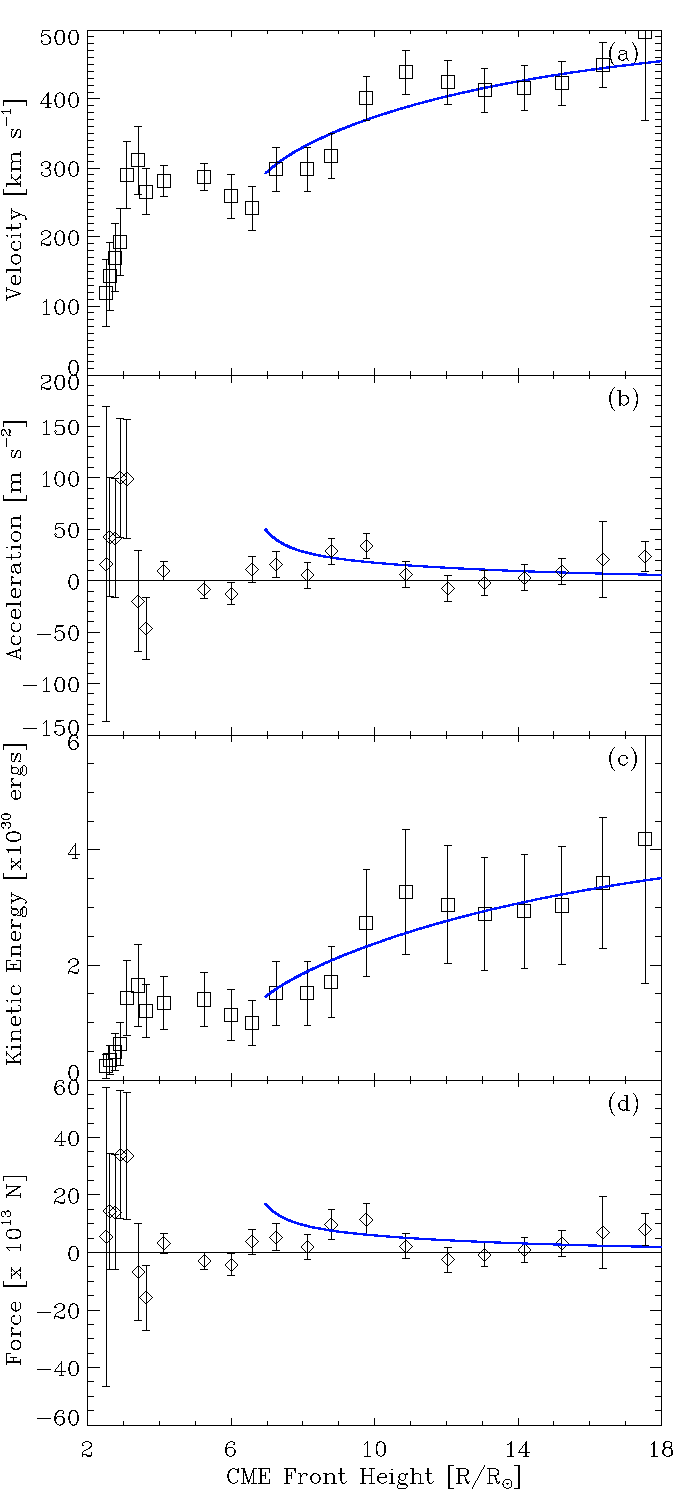
\includegraphics[scale=0.75, angle=0]{images/20081212_force_v2.pdf}
\caption[CME kinematics and energetics as a function of height]{(a) CME velocity as a function of heliocentric distance, including a fit to the data produced using an aerodynamic drag model beyond $\sim$7\,$R_{\odot}$ \citep{byrne2010}. (b) Acceleration of CME, including fit,  derived from the velocity data and fit. 
Panel (c) and (d) show the kinetic energy and force, respectively, both calculated using constant CME mass of $3.4\,\pm\,1.0\times10^{15}$\,g and kinematics results from (a) and (b). Also shown are the fits to energy and force produced from fits to velocity and acceleration.}
\label{fig:force_20081212}
\end{center}
\end{figure}
\clearpage

The CME kinetic energy was calculated using $E_{kin}=1/2M_{cme}v_{cme}^{2}$, where $M_{cme}$ is the final asymptotic mass of 3.4\,$\pm$\,1.0$\times$10$^{15}$\,g and $v_{cme}$ are the instantaneous velocity measurements, results of this calculation are shown in Figure~\ref{fig:force_20081212}(c). The kinetic energy shows 
an initial rise towards 6.3\,$\pm$\,3.7$\times$10$^{29}$\,ergs at $\sim$3\,$R_{\odot}$, beyond which it rises steadily to 4.2\,$\pm$\,2.5$\times$10$^{30}$\,ergs at $\sim$18\,$R_{\odot}$, these values are similar to those reported in \citet{vou00, vour2010} and \citet{emslie2004}. 

The total force on the CME was calculated using $F_{total}=M_{cme}a_{cme}$, where $M_{cme}$ is as above and $a_{cme}$ is taken from the instantaneous acceleration values. As shown in panel (d) of Figure~\ref{fig:force_20081212}, the force initially grows significantly, reaching a maximum value of 3.4\,$\pm$\,2.2$\times$10$^{14}$\,N at $\sim$3\,$R_
{\odot}$. The early rise and fall in acceleration (or force) is in agreement with a previous study of a CME observed to reach peak acceleration at $\sim$1.7\,$R_{\odot}$ after which it reaches a constant velocity beyond $\sim$3.4\,$R_{\odot}$ \citep{gallagher03}.  Such results are also found in a statistical study which shows that the majority of CMEs have peak acceleration in the low corona with a mean height of maximum acceleration at 1.5\,$R_{\odot}$ 
\citep{bein2011}. Similarly, observational studies by \citet{zhang2001} and \citet{zhang2004} also show early phase peak acceleration between 2--5\,$R_{\odot}$ and forces on the order of 10$^{15}$\,N and 10$^{12}$\,N, depending on whether the CME shows large initial acceleration or a slow, more gradual acceleration.

After this early peak, the force drops to an average value of 3.8$\pm$5.4$\times$10$^{13}$\,N at distances between 7--18\,$R_{\odot}$. It is apparent from Figure~\ref{fig:force_20081212}(a) that the velocity continues to increase beyond $7\,R_{\odot}$, implying that a positive radial force must be present. To clarify this, a fit to the velocity data using a model for solar wind drag on the CME beyond $7\,R_{\odot}$ (as outlined in \citet{byrne2010}) is shown in Figure~\ref{fig:force_20081212}(a). Although the data suggest a non-monotonic increase in velocity, the fit reveals that propagation is best described by a steadily increasing velocity between 7--18\,$R_{\odot}$. The acceleration and kinetic energy curves derived from this velocity fit are shown in Figure~\ref{fig:force_20081212}(b) and (c). In Figure~\ref{fig:force_20081212}(d), the curve for the force derived from the velocity fit initially deviates from the data at $\sim$7\,$R_{\odot}$, however beyond this distance there is good agreement with the data and the derived force is entirely positive.  This suggests that the solar wind exerts a positive aerodynamic drag force on the CME, resulting in a velocity that approaches the asymptotic solar wind speed at large heliospheric distances. 

%\subsection{Mechanical Energy}\label{sec:20}

\subsection{Forces}\label{sec:21}

It should be noted that Figure~\ref{fig:20081212_mass_ht} shows an overall exponential increase in CME mass with height which could be interpreted as the CME rapidly gaining mass as it propagates. Care should be taken with this interpretation since this apparent exponential mass increase is almost certainly due to the CME moving into the field of view, therefore allowing us to measure more of its mass content; such an interpretation is in agreement with similar assertions made in \citet{vour2010}. It is difficult to distinguish between actual CME mass growth and an apparent growth due to more of the CME being observed. If the initial early rise in CME mass is assumed to be an observational artifact then we can interpret the CME mass to be in the range of (3--3.5)$\times$10$^{15}$\,g for most of its early propagation i.e., the CME already has such a mass before launch and does not acquire more mass (via inflows or otherwise) during propagation.
Such an interpretation is in agreement with CME mass measurements calculated from dimmings in \emph{STEREO} Extreme Ultraviolet Image(EUVI) images, which show the mass calculated from EUV images to be approximately equal to CME mass in COR2 images,  $m_{EUVI}/m_{COR2} =1.1\pm0.3$  \citep{aschw09}. Once the CME bubble is in the field of view at $\sim$10\,$R_{\odot}$ the mass in its entirety can be measured and the increase beyond this point, if any, is slow and steady, Figure~\ref{fig:20081212_mass_ht}.

The early stages of CME propagation are dominated by a sharp rise to a peak force of 3.4\,$\pm$\,2.2$\times$10$^{14}$\,N at $\sim$3\,$R_{\odot}$ followed by a sharp decline, Figure~\ref{fig:force_20081212}(d). The catastrophe model \citep{forbes1991,forbes1995,lin2000}, magnetic breakout model \citep{antio99,lynch2008}, and toroidal instability model \citep{chen1996,kleim2006} employ a number of forces acting on the CME to produce an over all acceleration into interplanetary space. For example, the toroidal instability model used by \citet{chen1996} uses a Lorentz hoop force (or Lorentz self-force), solar wind drag, and gravity to provide a net force acting on the CME between 2--3\,$R_{\odot}$ that quickly 
rises to a peak total force of $\sim$10$^{16}$\,N and then falls rapidly.

If we assume that the peak force observed for the 2008 December 12 CME is the net force due to similar forces used in the above models, such as the solar wind drag, gravity, and some form of magnetic CME driver e.g., a $\vec{J}\,\times\,\vec{B}$ force, we may estimate their relative contribution. The force due to solar wind drag on the CME is given by
\begin{equation}
\vec{F}_d=-\frac{1}{2}C_{d}\rho_{sw}A_{cme}(\vec{v}-\vec{v}_{sw})\mid\,\vec{v}-\vec{v}_{sw}\mid
\end{equation}
where $M_{cme}$ is the CME mass, $\vec{v}$ is the CME velocity, $C_{d}$ is the drag coefficient, $\rho_{sw}$ is the solar wind mass density, $A_{cme}$ is the CME area exposed to solar wind drag and $\vec{v}_{sw}$ is the solar wind velocity \citep{malo10}. To estimate the effects of this force we use $\rho_{sw}=n_{p}m_{p}$, where $m_{p}$ is proton mass, and assume ionization fraction of $\chi$\,=\,1 such that $n_{p}=n_{e}$\,$[cm^{-3}]$. Electron density, and hence proton density, is then given by an interplanetary density model derived from a special solution of the Parker solar wind equation \citep{Mann1999}, solar wind velocity values as a function of height are also determined using this model. $A_{cme}$ is estimated using the expression derived in \citet{byrne2010} for latitudinal angular width of the CME as a function of height, $\psi(r)=26r^{0.22}$. This is used to derive an arc length of the CME front and, as above, making the assumption $\phi=2\psi$, the two arc lengths derived from these angles then give the surface that the solar wind acts on, thus $A_{cme}$\,=\,1352$r^{2.44}$. Setting the drag coefficient $C_{d}=1$, and using the \citet{Mann1999} model to derive a density and a solar wind velocity of 2.3$\times$10$^{5}$\,cm$^{-3}$  and 70\,km\,s$^{-1}$, respectively, equation [1] then gives a force of $\vec{F}_{d}=-8.0\times10^{12}\,\hat{r}\,$\,N for solar wind drag at $\sim$3\,$R_{\odot}$, where $\hat{r}$ is a unit vector in the positive radial direction. 

A simple estimate of force due to gravity is given by $\vec{F}_{g}=GM_{\odot}M_{cme}/\vec{r}\,^2$, where $G$ is the universal gravitational constant, $M_{\odot}$ is solar mass, $M_{cme}$ is CME mass, and $\vec{r}$ is a heliocentric position vector\footnote{Ideally the heliocentric distance of the CME centre of mass would be used here. However an unknown amount of mass is obscured by the coronagraphs occulting disk, making the mass distribution and hence COM difficult to determine. Thus the CME front height is used in the calculation of force due to gravity}. Given a CME mass of 3.4$\times$10$^{15}$\,g the force due to gravity at a heliocentric distance of 3\,$R_{\odot}$ is $\vec{F}_{g}=-1.0\times10^
{14}\,\hat{r}$\,N. From the MHD momentum conservation equation (equation~\ref{eqn:mhd_momentum}), the only remaining contribution is due to some form of magnetic CME driver, $F_{mag}$, which is estimated using 
\begin{equation}
\vec{F}_{mag}= \vec{F}_{total}-\vec{F}_{d}-\vec{F}_{g}
\end{equation}
(the pressure gradient in the CME equation of motion is assumed to be negligable and has been omitted here). Using the above values, the total magnetic contribution to CME force is calculated to be $\vec{F}_{mag}\approx4.5\times10^{14}\,\hat{r}$\,N at 3\,$R_{\odot}$, indicating that this is the largest driver of CMEs at low coronal heights. Lorentz force dominated dynamics in early phase CME propagation are reported in \citet{bein2011}, in which a statistical study of a large sample of CMEs in EUVI, COR1, and COR2 indicated an early phase acceleration for the majority of CMEs that is attributable to a Lorentz force.  A similar result of an observational study by \citet{vrs06} found that the Lorentz force plays a dominant role within a few solar radii. It should be noted that although we have labelled the force $F_{mag}$, there is no distinction on the exact form of this force e.g., whether it is magnetic pressure, magnetic tension, or a Lorentz self-force that acts as the driver. Also, any non-radial motion of the CME, such as that described in \citet{byrne2010}, is not taken into account here; any force estimates are purely radial in direction.


 \section{Conclusion} \label{bozomath}
 The \emph{STEREO} COR1/2 coronagraphs have been used to determine the mass development of the 2008 December 12 CME. Knowledge of the longitudinal propagation angle of the CME allowed for a significant reduction in the mass uncertainty, giving a final estimate of 3.4\,$\pm$\,1.0$\times$10$^{15}$\,g. Using kinematics results of a previous study \citep{byrne2010}, the velocity and acceleration of the CME were combined with the mass measurements to determine the kinetic energy and total force on the CME. The early phase propagation of the CME was found to be dominated by a force of peak magnitude of 3.4\,$\pm$\,2.2$\times$10$^{14}$\,N at $\sim$3.0\,$R_{\odot}$, after which the magnitude declines 
rapidly and settles to and average of 3.8 $\pm$ 5.4$\times$10$^{13}$\,N. This early rise and fall in total force (or acceleration) is in agreement with previous observations of CME kinematics \citep{gallagher03, bein2011}. Similarly results of observational studies by \citet{zhang2001} and \citet{zhang2004} also show early phase peak acceleration between 2--5\,$R_{\odot}$ and forces on the order of 10$^{15}$\,N and 10$^{12}$\,N. The kinetic energy shows an initial rise steadily to 4.2\,$\pm$\,2.5$\times$10$^{30}$\,ergs at $\sim$18\,$R_{\odot}$, such order of magnitudes are similar to those reported in \citet{vou00,emslie2004} and are typical of CME kinetic energies \citep{vour2010}.

Such CME kinematics and dynamics property estimates cannot be carried out when unknown propagation angle hinders an accurate calculation of CME mass, hence adding unacceptable uncertainty to any subsequent calculations. This highlights the need for similar studies using the \emph{STEREO} mission's ability to accurately determine the physical properties of CMEs, such as mass, with remarkably reduced uncertainty. Increasing the accuracy of force estimates of other well studied CMEs will allow for a more complete view of the magnitude of the forces influencing CME propagation and will allow model parameters to be more accurately constrained.




